\subsection{UC21 - Visualizzazione dashboard fornita dal plug-in}
\begin{figure}[H]
	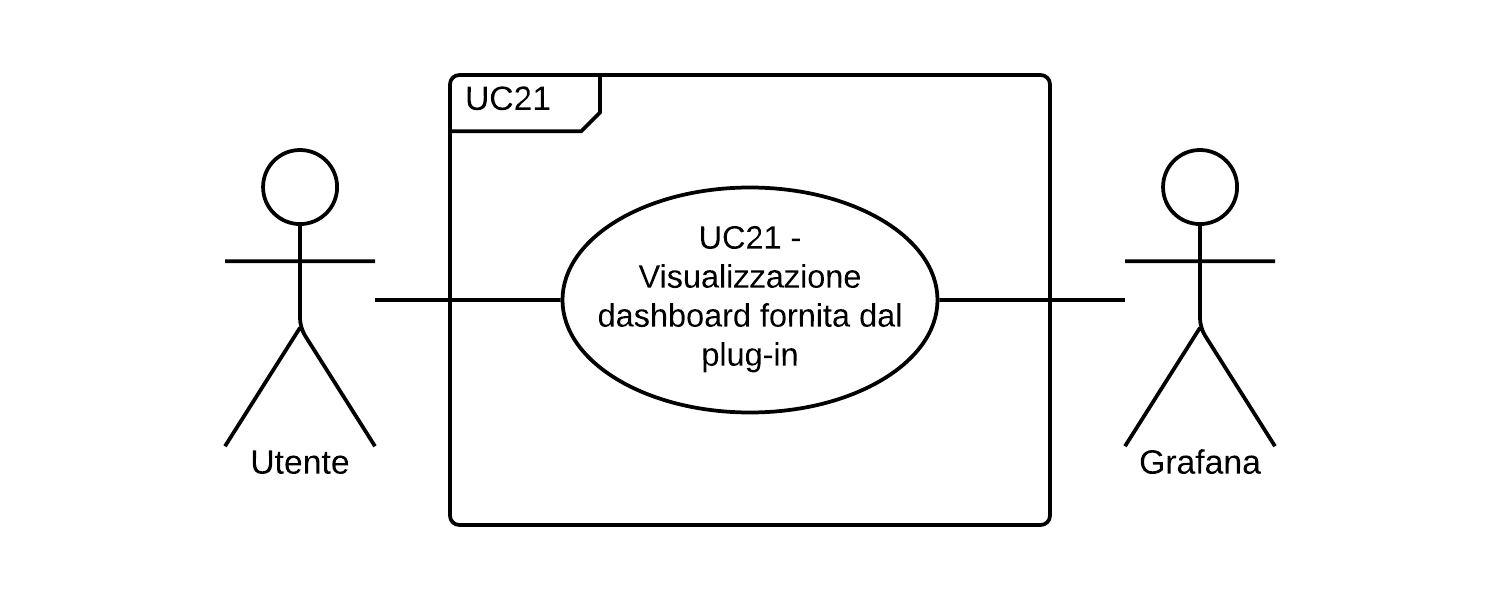
\includegraphics{img/UC21_-_Visualizzazione_dashboard_fornita_dal_plug-_in.png}
	\caption{Diagramma degli use case di UC21}
\end{figure}
\begin{itemize}
	\item \textbf{Codice identificativo}: UC21;
	\item \textbf{Titolo}: visualizzazione dashboard\glosp fornita dal plug-in;
	\item \textbf{Attori primari}: utente;
	\item \textbf{Attori secondari}: Grafana\glo;
	\item \textbf{Descrizione}: l'utente visualizza la dashboard\glosp predefinita fornita dal plug-in contenente dei pannelli e delle impostazioni preconfigurate per introdurre le funzionalità fornite dal plug-in stesso;
	\item \textbf{Precondizioni}: l'utente è autenticato nel sistema software Grafana\glosp ed ha abilitato il plug-in;
	\item \textbf{Postcondizioni}: l'utente visualizza correttamente la dashboard\glosp predefinita fornita dal plug-in;
	\item \textbf{Scenario principale}: l'utente, utilizzando il menù di navigazione di Grafana\glo, apre e visualizza la dashboard\glosp predefinita fornita dal plug-in.
\end{itemize} 
